%!TEX root = ../stoeter_sourcecount.tex
\section{Model Selection}%
\label{sec:hyperparameters}
% Describe popular Input representations and why MFCCs are not used in
% experiments, MEL  STFT, LOG STFT
%
% * All mixtures have the same 0dB SNR to all others
% * Trained on 20.020 Libri Speech Mixtures
% * Number Speakers [0, 1, 2, ..., 10]
% * Temporal Context (5s)
% * Different Input Representations (STFT 400, MEL40, log(STFT + 1)))
% * Different Output Objectives (classification, regression, p-regression)
%
% * --> Fix Input Representation to STFT because of little influence
% * --> Fix Output Objective to Classification for best overall performance

In this section we evaluate of three configurations of our proposed architectures, introduced in Section~\ref{sec:supervised_learning}.
Besides the architecture we investigate different input representations as well as the three proposed output distributions (see Section~\ref{sec:problem_formulation}).
The goal of this is to determine the effect of these parameters and fix them to select a final trained network (model) based on these parameters.
\par
% maybe move this down to "model comparison?"
To allow for a controlled test environment and at the same time limit the number of training iterations, we fix certain parameters:
In this experiment all speakers were mixed to 0~dB SNR.\@
Furthermore, the input duration \(D\) was fixed to five seconds.
For all experimental parameters we repeated the training three times with different random seeds for each run and report averaged results to minimize random effects caused by early stopping.
We used the \emph{LibriSpeech} dataset for both training and validation and
performed evaluation of all models on \(T_{\textrm{test}} = 5720\) unique and unseen speaker mixtures from \emph{LibriSpeech test-clean} set with \(k_{\max} = 10\).
\par
% \subsection{Input Representations}
% Up to date, most discriminative models for speech applications rely on  time-frequency (TF) magnitude representations.
% This is because, compared to raw time-domain models, TF models allow for faster training due to less data redundancy leading to generally fewer trainable parameters or shorter training duration.
Several well established input representations were evaluated in~\cite{stoeter17} such as (linear or logarithmically scaled) Short-time Fourier transform (STFT), Mel filter bank outputs (MEL), Mel Frequency Cepstral Coefficients (MFCC) representations, typically chosen for speech applications.

% \begin{table}
% \caption{Speech related Input representations}
% \label{tab:inputrep}
%   \centering
% \begin{tabular}{rll}
% \toprule
% References & Task & Representation \\
% \midrule
% \cite{geiger13, hagerer17} & Overlap Detection/VAD & MFCC \\
% \cite{Graves13, sainath15, marchi17} & ASR & MEL \\
% \cite{amodei16} & ASR & STFT \\
% \cite{schluter15, schluter16} & Singing Voice AD & \(\log(1 + \mathbf{X})\) \\
% \bottomrule
% \end{tabular}
% \end{table}

% As for the task of estimating the number of speakers, we assume that a fine frequency resolution is needed to discriminate time frequency bins with overlapped speech segments from those that only belong to a single speaker.
Even though MFCCs are used in related tasks and are included in our baseline evaluations, they are known to perform poorly when used in CNNs~\cite{Seltzer13}.
This is why we decided to not to use the MFCCs as an input for the proposed architectures.
The remaining input representations are identical to those listed in~\cite{stoeter17}:

\noindent\textbf{1) STFT}: magnitude of the Short-time Fourier transform computed using Hann-windows.
A frame length of 25~ms has been used.
The resulting input is \(X \in \mathbb{R}^{500 \times 201}\).\\
\textbf{2) LOGSTFT}: logarithmically scaled magnitudes from STFT representation using \(\log(1 + STFT)\).
The resulting input is \(X \in \mathbb{R}^{500 \times 201}\).\\
\textbf{3) MEL}: compute mapping from the STFT output directly onto Mel basis using 40 triangular filters.
The resulting input is \(X \in \mathbb{R}^{500 \times 40}\).
\par
Before feature transformation, all input files were re-sampled to 16 kHz sampling rate. All features are computed using a hop size of 10~ms.

\subsection{Metric}%
\label{ssec:metrics}

Whereas the intermediate output \(y\) is treated as either a classification or a regression problem (see Section~\ref{sec:problem_formulation}) we evaluate the final output \(\cardinality \) as a discrete regression problem.
We therefore employ the mean absolute error (MAE) being the most accessible metric, also commonly used for other count related tasks (c.f.~\cite{zhang15, Rezatofigh16}).
Since the MAE is based on the true count \(\cardinality \), we also present the individual mean absolute count error as:

\begin{equation}
  \mbox{MAE}(k) = \frac{1}{T_{\textrm{test}}} \sum_{t=1}^{T_\textrm{test}}\left| \hat{k} - k \right|.
\end{equation}

which is then averaged

\begin{equation}
  \mbox{MAE} = \frac{1}{k_{\max}} \sum_{k=0}^{k_{\max}} \mbox{MAE}(k).
\end{equation}

% * Mean Speaker Count Distance
% * Accuracy
% * Accuracy +/- 1
% * Response

\subsection{Model Comparison}%
\label{ssec:model_comparsion}

% \begin{figure*}[ht!]
%   \begin{subfigure}[b]{0.30\textwidth}
%       \centering
%       \begin{adjustbox}{width=\textwidth}
%         % This file was created by matplotlib2tikz v0.6.13.
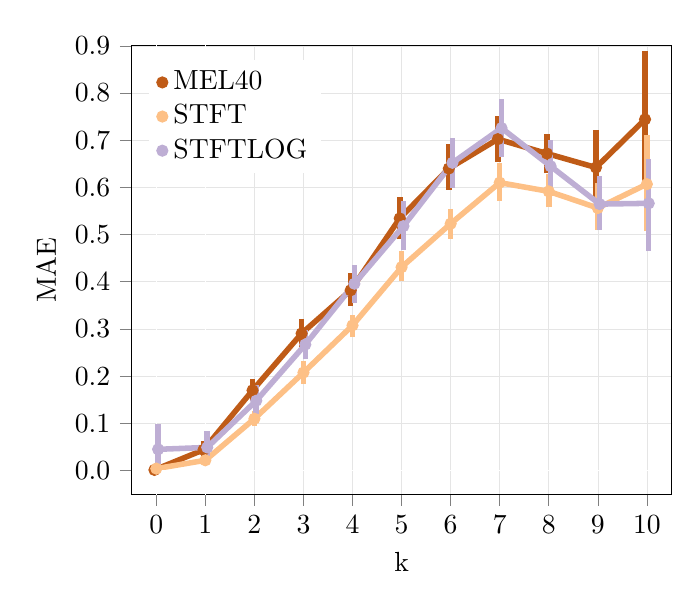
\begin{tikzpicture}

% colors from colorbrewer Set3
\definecolor{color0}{rgb}{0.917647058823529,0.917647058823529,0.949019607843137}
\definecolor{color1}{RGB}{191,91,23}
\definecolor{color3}{RGB}{190,174,212}
\definecolor{color2}{RGB}{253,192,134}

\begin{axis}[
xlabel={k},
ylabel={MAE},
xmin=-0.5, xmax=10.5,
ymin=-0.05, ymax=0.9,
ytick={-0.1,0,0.1,0.2,0.3,0.4,0.5,0.6,0.7,0.8,0.9},
yticklabels={0.0,0.0,0.1,0.2,0.3,0.4,0.5,0.6,0.7,0.8,0.9},
xtick distance=1,
tick align=outside,
tick pos=left,
ymajorgrids,
xmajorgrids,
grid style={line width=.1pt, draw=gray!20},
major grid style={line width=.2pt,draw=gray!20},
axis line style={black},
legend style={at={(0.03,0.97)}, anchor=north west, draw=none, fill==gray!0},
legend cell align={left},
legend entries={{MEL40},{STFT},{STFTLOG}}
]
\addplot [only marks, draw=color1, fill=color1, colormap/blackwhite]
table{%
x                      y
-3.750000000000001e-02 +1.282051285115891e-03
+9.625000000000000e-01 +4.378956559182671e-02
+1.962500000000000e+00 +1.698966412812240e-01
+2.962500000000000e+00 +2.904593644946708e-01
+3.962500000000000e+00 +3.819121458168999e-01
+4.962500000000000e+00 +5.342699044052212e-01
+5.962500000000000e+00 +6.399449048893949e-01
+6.962500000000000e+00 +7.022138688498571e-01
+7.962500000000000e+00 +6.717410322614437e-01
+8.962500000000000e+00 +6.421099899821276e-01
+9.962500000000000e+00 +7.441498321916922e-01
};
\addplot [line width=2.00pt, color1, forget plot]
table {%
-0.0375 0.00128205128511589
0.9625 0.0437895655918267
1.9625 0.169896641281224
2.9625 0.290459364494671
3.9625 0.3819121458169
4.9625 0.534269904405221
5.9625 0.639944904889395
6.9625 0.702213868849857
7.9625 0.671741032261444
8.9625 0.642109989982128
9.9625 0.744149832191692
};
\addplot [line width=2.00pt, color1, forget plot]
table {%
-0.0375 0.0002991452993443
-0.0375 0.00290598291171611
};
\addplot [line width=2.00pt, color1, forget plot]
table {%
0.9625 0.0292021391029433
0.9625 0.0628356254969424
};
\addplot [line width=2.00pt, color1, forget plot]
table {%
1.9625 0.148319336806491
1.9625 0.1932881148387
};
\addplot [line width=2.00pt, color1, forget plot]
table {%
2.9625 0.260852964485001
2.9625 0.322079899352019
};
\addplot [line width=2.00pt, color1, forget plot]
table {%
3.9625 0.348403317338685
3.9625 0.418488374525981
};
\addplot [line width=2.00pt, color1, forget plot]
table {%
4.9625 0.490396980724153
4.9625 0.580383148183019
};
\addplot [line width=2.00pt, color1, forget plot]
table {%
5.9625 0.59489899164649
5.9625 0.690870064470585
};
\addplot [line width=2.00pt, color1, forget plot]
table {%
6.9625 0.654216791062228
6.9625 0.75059524217121
};
\addplot [line width=2.00pt, color1, forget plot]
table {%
7.9625 0.629482719495514
7.9625 0.712939632123146
};
\addplot [line width=2.00pt, color1, forget plot]
table {%
8.9625 0.5712637464472
8.9625 0.720740745223197
};
\addplot [line width=2.00pt, color1, forget plot]
table {%
9.9625 0.603217593893058
9.9625 0.889956860029537
};
\addplot [only marks, draw=color2, fill=color2, colormap/blackwhite]
table{%
x                      y
+0.000000000000000e+00 +4.017094149429383e-03
+1.000000000000000e+00 +2.165466058294658e-02
+2.000000000000000e+00 +1.097760553809459e-01
+3.000000000000000e+00 +2.075775420503098e-01
+4.000000000000000e+00 +3.075366057808496e-01
+5.000000000000000e+00 +4.309067676908769e-01
+6.000000000000000e+00 +5.230027550672368e-01
+7.000000000000000e+00 +6.100250622981175e-01
+8.000000000000000e+00 +5.915135611073551e-01
+9.000000000000000e+00 +5.562738505022561e-01
+1.000000000000000e+01 +6.068181814770105e-01
};
\addplot [line width=2.00pt, color2, forget plot]
table {%
0 0.00401709414942938
1 0.0216546605829466
2 0.109776055380946
3 0.20757754205031
4 0.30753660578085
5 0.430906767690877
6 0.523002755067237
7 0.610025062298117
8 0.591513561107355
9 0.556273850502256
10 0.60681818147701
};
\addplot [line width=2.00pt, color2, forget plot]
table {%
0 0.00141025642932265
0 0.00777884649395501
};
\addplot [line width=2.00pt, color2, forget plot]
table {%
1 0.015104780559566
1 0.0292981881977767
};
\addplot [line width=2.00pt, color2, forget plot]
table {%
2 0.0935389754212398
2 0.126616063651554
};
\addplot [line width=2.00pt, color2, forget plot]
table {%
3 0.184214762288727
3 0.232517668003831
};
\addplot [line width=2.00pt, color2, forget plot]
table {%
4 0.283712317184782
4 0.329804048656288
};
\addplot [line width=2.00pt, color2, forget plot]
table {%
5 0.401557044723647
5 0.465348019600485
};
\addplot [line width=2.00pt, color2, forget plot]
table {%
6 0.490907942142724
6 0.554963269541031
};
\addplot [line width=2.00pt, color2, forget plot]
table {%
7 0.571706349037544
7 0.650759191716972
};
\addplot [line width=2.00pt, color2, forget plot]
table {%
8 0.557388451102525
8 0.628085083916509
};
\addplot [line width=2.00pt, color2, forget plot]
table {%
9 0.510563413293006
9 0.60849158311509
};
\addplot [line width=2.00pt, color2, forget plot]
table {%
10 0.507567340790322
10 0.711869740708408
};
\path [draw=white, fill opacity=0] (axis cs:0,-0.0552693502854651)
--(axis cs:0,0.934967631949299);

\path [draw=white, fill opacity=0] (axis cs:1,-0.0552693502854651)
--(axis cs:1,0.934967631949299);

\path [draw=white, fill opacity=0] (axis cs:-0.5,0)
--(axis cs:10.5,0);

\path [draw=white, fill opacity=0] (axis cs:-0.5,1)
--(axis cs:10.5,1);

\addplot [only marks, draw=color3, fill=color3, colormap/blackwhite]
table{%
x                      y
+3.750000000000001e-02 +4.491453003381084e-02
+1.037500000000000e+00 +4.894127914890618e-02
+2.037500000000000e+00 +1.479328153983824e-01
+3.037500000000000e+00 +2.669022376087070e-01
+4.037500000000000e+00 +3.958656320969263e-01
+5.037500000000000e+00 +5.179225227638933e-01
+6.037500000000000e+00 +6.520202012977215e-01
+7.037500000000000e+00 +7.256892264536648e-01
+8.037500000000000e+00 +6.448818897898534e-01
+9.037500000000000e+00 +5.645342315434071e-01
+1.003750000000000e+01 +5.662037049329240e-01
};
\addplot [line width=2.00pt, color3, forget plot]
table {%
0.0375 0.0449145300338108
1.0375 0.0489412791489062
2.0375 0.147932815398382
3.0375 0.266902237608707
4.0375 0.395865632096926
5.0375 0.517922522763893
6.0375 0.652020201297722
7.0375 0.725689226453665
8.0375 0.644881889789853
9.0375 0.564534231543407
10.0375 0.566203704932924
};
\addplot [line width=2.00pt, color3, forget plot]
table {%
0.0375 0.00563675216719425
0.0375 0.0978333334729233
};
\addplot [line width=2.00pt, color3, forget plot]
table {%
1.0375 0.0240973587901605
1.0375 0.083095393889988
};
\addplot [line width=2.00pt, color3, forget plot]
table {%
2.0375 0.119852497411666
2.0375 0.180880703087784
};
\addplot [line width=2.00pt, color3, forget plot]
table {%
3.0375 0.236119944983176
3.0375 0.298233213870577
};
\addplot [line width=2.00pt, color3, forget plot]
table {%
4.0375 0.354053618227044
4.0375 0.434679154426463
};
\addplot [line width=2.00pt, color3, forget plot]
table {%
5.0375 0.46628033370452
5.0375 0.5704150723004
};
\addplot [line width=2.00pt, color3, forget plot]
table {%
6.0375 0.599070247832217
6.0375 0.705386820743399
};
\addplot [line width=2.00pt, color3, forget plot]
table {%
7.0375 0.663815792690194
7.0375 0.786649962138935
};
\addplot [line width=2.00pt, color3, forget plot]
table {%
8.0375 0.588227250151147
8.0375 0.700395887889496
};
\addplot [line width=2.00pt, color3, forget plot]
table {%
9.0375 0.508768798929406
9.0375 0.623634119981668
};
\addplot [line width=2.00pt, color3, forget plot]
table {%
10.0375 0.464126683435331
10.0375 0.659747474216276
};
\end{axis}

\end{tikzpicture}

%       \end{adjustbox}
%       \caption{by feature representations.}%
%       \label{fig:ssec:exp_fixed_gains/A}
%   \end{subfigure}\hfill%
%   \begin{subfigure}[b]{0.30\textwidth}
%       \centering
%       \begin{adjustbox}{width=\textwidth}
%         % This file was created by matplotlib2tikz v0.6.13.
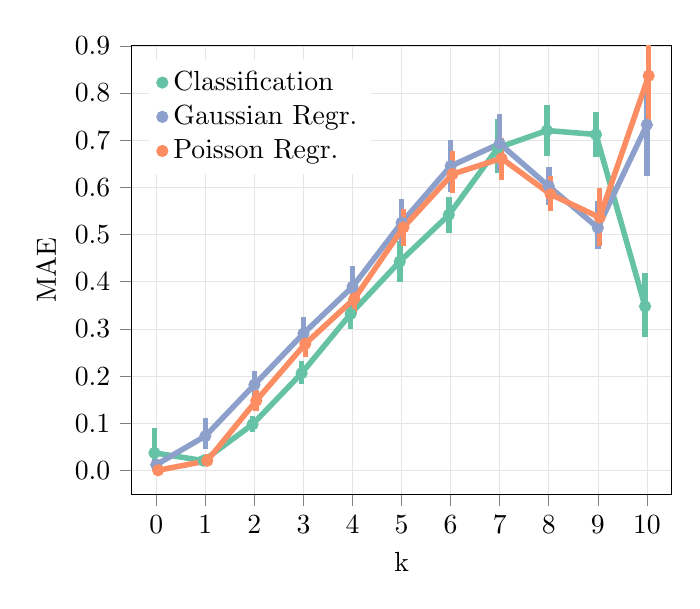
\begin{tikzpicture}

\definecolor{color0}{rgb}{0.917647058823529,0.917647058823529,0.949019607843137}
\definecolor{color1}{RGB}{102,194,165}
\definecolor{color3}{RGB}{252,141,98}
\definecolor{color2}{RGB}{141,160,203}

\begin{axis}[
xlabel={k},
ylabel={MAE},
xmin=-0.5, xmax=10.5,
ymin=-0.05, ymax=0.9,
ytick={-0.1,0,0.1,0.2,0.3,0.4,0.5,0.6,0.7,0.8,0.9},
yticklabels={0.0,0.0,0.1,0.2,0.3,0.4,0.5,0.6,0.7,0.8,0.9},
xtick distance=1,
tick align=outside,
tick pos=left,
ymajorgrids,
xmajorgrids,
axis line style={black},
grid style={line width=.1pt, draw=gray!20},
major grid style={line width=.2pt,draw=gray!20},
legend style={at={(0.03,0.97)}, anchor=north west, draw=none, fill==gray!0},
legend entries={{Classification},{Gaussian Regr.},{Poisson Regr.}},
legend cell align={left}
]
\addplot [only marks, draw=color1, fill=color1, colormap/blackwhite]
table{%
x                      y
-3.750000000000001e-02 +3.735042735042735e-02
+9.625000000000000e-01 +2.086880593756822e-02
+1.962500000000000e+00 +9.780361757105942e-02
+2.962500000000000e+00 +2.061248527679623e-01
+3.962500000000000e+00 +3.319121447028424e-01
+4.962500000000000e+00 +4.427415921668795e-01
+5.962500000000000e+00 +5.417355371900826e-01
+6.962500000000000e+00 +6.838345864661655e-01
+7.962500000000000e+00 +7.204724409448819e-01
+8.962500000000000e+00 +7.120987654320987e-01
+9.962500000000000e+00 +3.478956228956228e-01
};
\addplot [line width=2.00pt, color1, forget plot]
table {%
-0.0375 0.0373504273504274
0.9625 0.0208688059375682
1.9625 0.0978036175710594
2.9625 0.206124852767962
3.9625 0.331912144702842
4.9625 0.44274159216688
5.9625 0.541735537190083
6.9625 0.683834586466165
7.9625 0.720472440944882
8.9625 0.712098765432099
9.9625 0.347895622895623
};
\addplot [line width=2.00pt, color1, forget plot]
table {%
-0.0375 0.00153739316239316
-0.0375 0.0895363247863248
};
\addplot [line width=2.00pt, color1, forget plot]
table {%
0.9625 0.0127919668194717
0.9625 0.0316961362148003
};
\addplot [line width=2.00pt, color1, forget plot]
table {%
1.9625 0.0817797157622739
1.9625 0.114736218776916
};
\addplot [line width=2.00pt, color1, forget plot]
table {%
2.9625 0.182602080879466
2.9625 0.231887514723204
};
\addplot [line width=2.00pt, color1, forget plot]
table {%
3.9625 0.29969315245478
3.9625 0.365779500430663
};
\addplot [line width=2.00pt, color1, forget plot]
table {%
4.9625 0.399341209025117
4.9625 0.485740740740741
};
\addplot [line width=2.00pt, color1, forget plot]
table {%
5.9625 0.502793847566575
5.9625 0.579757805325987
};
\addplot [line width=2.00pt, color1, forget plot]
table {%
6.9625 0.631313700918964
6.9625 0.745908521303258
};
\addplot [line width=2.00pt, color1, forget plot]
table {%
7.9625 0.66682195975503
7.9625 0.773801399825022
};
\addplot [line width=2.00pt, color1, forget plot]
table {%
8.9625 0.663826038159372
8.9625 0.758792368125701
};
\addplot [line width=2.00pt, color1, forget plot]
table {%
9.9625 0.283256523569024
9.9625 0.418800505050505
};
\addplot [only marks, draw=color2, fill=color2, colormap/blackwhite]
table{%
x                      y
+0.000000000000000e+00 +1.235042760510825e-02
+1.000000000000000e+00 +7.290984498750833e-02
+2.000000000000000e+00 +1.817398789856169e-01
+3.000000000000000e+00 +2.903023165133264e-01
+4.000000000000000e+00 +3.893195516533322e-01
+5.000000000000000e+00 +5.250319321950276e-01
+6.000000000000000e+00 +6.450872368282742e-01
+7.000000000000000e+00 +6.927318334579468e-01
+8.000000000000000e+00 +6.023184604114956e-01
+9.000000000000000e+00 +5.145679036776225e-01
+1.000000000000000e+01 +7.327020216319297e-01
};
\addplot [line width=2.00pt, color2, forget plot]
table {%
0 0.0123504276051083
1 0.0729098449875083
2 0.181739878985617
3 0.290302316513326
4 0.389319551653332
5 0.525031932195028
6 0.645087236828274
7 0.692731833457947
8 0.602318460411496
9 0.514567903677623
10 0.73270202163193
};
\addplot [line width=2.00pt, color2, forget plot]
table {%
0 0.00534081213764795
0 0.0241025645566535
};
\addplot [line width=2.00pt, color2, forget plot]
table {%
1 0.0466262830175563
1 0.110413665477342
};
\addplot [line width=2.00pt, color2, forget plot]
table {%
2 0.155333763578286
2 0.211202626282142
};
\addplot [line width=2.00pt, color2, forget plot]
table {%
3 0.257034745460583
3 0.324860619132717
};
\addplot [line width=2.00pt, color2, forget plot]
table {%
4 0.34692829568353
4 0.432953272768193
};
\addplot [line width=2.00pt, color2, forget plot]
table {%
5 0.478991059346331
5 0.574425296684106
};
\addplot [line width=2.00pt, color2, forget plot]
table {%
6 0.590747243298425
6 0.699374426702658
};
\addplot [line width=2.00pt, color2, forget plot]
table {%
7 0.634959278139803
7 0.754830837696791
};
\addplot [line width=2.00pt, color2, forget plot]
table {%
8 0.562505469305648
8 0.6433584856987
};
\addplot [line width=2.00pt, color2, forget plot]
table {%
9 0.468725030223529
9 0.570103260063463
};
\addplot [line width=2.00pt, color2, forget plot]
table {%
10 0.624493893070353
10 0.840917507157558
};
% \path [draw=white, fill opacity=0] (axis cs:0,-0.0600185928210457)
% --(axis cs:0,1.00006922752411);
%
% \path [draw=white, fill opacity=0] (axis cs:1,-0.0600185928210457)
% --(axis cs:1,1.00006922752411);
%
% \path [draw=white, fill opacity=0] (axis cs:-0.5,0)
% --(axis cs:10.5,0);
%
% \path [draw=white, fill opacity=0] (axis cs:-0.5,1)
% --(axis cs:10.5,1);

\addplot [only marks, draw=color3, fill=color3, colormap/blackwhite]
table{%
x                      y
+3.750000000000001e-02 +5.128205128205128e-04
+1.037500000000000e+00 +2.060685439860293e-02
+2.037500000000000e+00 +1.480620155038760e-01
+3.037500000000000e+00 +2.685119748723989e-01
+4.037500000000000e+00 +3.640826873385014e-01
+5.037500000000000e+00 +5.153256704980842e-01
+6.037500000000000e+00 +6.281450872359963e-01
+7.037500000000000e+00 +6.613617376775270e-01
+8.037500000000000e+00 +5.853455818022747e-01
+9.037500000000000e+00 +5.362514029180696e-01
+1.003750000000000e+01 +8.365740740740741e-01
};
\addplot [line width=2.00pt, color3, forget plot]
table {%
0.0375 0.000512820512820513
1.0375 0.0206068543986029
2.0375 0.148062015503876
3.0375 0.268511974872399
4.0375 0.364082687338501
5.0375 0.515325670498084
6.0375 0.628145087235996
7.0375 0.661361737677527
8.0375 0.585345581802275
9.0375 0.53625140291807
10.0375 0.836574074074074
};
\addplot [line width=2.00pt, color3, forget plot]
table {%
0.0375 0.000170940170940171
0.0375 0.000982905982905983
};
\addplot [line width=2.00pt, color3, forget plot]
table {%
1.0375 0.0122647893473041
1.0375 0.0345797860729098
};
\addplot [line width=2.00pt, color3, forget plot]
table {%
2.0375 0.12656976744186
2.0375 0.169559646856158
};
\addplot [line width=2.00pt, color3, forget plot]
table {%
3.0375 0.240591872791519
3.0375 0.298862387122104
};
\addplot [line width=2.00pt, color3, forget plot]
table {%
4.0375 0.332558139534884
4.0375 0.39405684754522
};
\addplot [line width=2.00pt, color3, forget plot]
table {%
5.0375 0.476749680715198
5.0375 0.554259259259259
};
\addplot [line width=2.00pt, color3, forget plot]
table {%
6.0375 0.587143021120294
6.0375 0.676090449954086
};
\addplot [line width=2.00pt, color3, forget plot]
table {%
7.0375 0.614816207184628
7.0375 0.704314954051796
};
\addplot [line width=2.00pt, color3, forget plot]
table {%
8.0375 0.549119641294838
8.0375 0.623103674540682
};
\addplot [line width=2.00pt, color3, forget plot]
table {%
9.0375 0.475597081930415
9.0375 0.597627384960718
};
\addplot [line width=2.00pt, color3, forget plot]
table {%
10.0375 0.727001262626263
10.0375 0.951883417508417
};
\end{axis}

\end{tikzpicture}

%       \end{adjustbox}
%       \caption{by output distribution.}%
%       \label{fig:ssec:exp_fixed_gains/B}
%   \end{subfigure}\hfill%
%   \begin{subfigure}[b]{0.30\textwidth}
%       \centering
%       \begin{adjustbox}{width=\textwidth}
%         % This file was created by matplotlib2tikz v0.6.13.
\begin{tikzpicture}

\definecolor{color0}{rgb}{0.917647058823529,0.917647058823529,0.949019607843137}

\begin{axis}[
xlabel={k},
ylabel={MAE},
xmin=-0.5, xmax=10.5,
ymin=-0.05, ymax=0.9,
ytick={-0.1,0,0.1,0.2,0.3,0.4,0.5,0.6,0.7,0.8,0.9},
yticklabels={0.0,0.0,0.1,0.2,0.3,0.4,0.5,0.6,0.7,0.8,0.9},
xtick distance=1,
tick align=outside,
tick pos=left,
ymajorgrids,
xmajorgrids,
axis line style={black},
grid style={line width=.1pt, draw=gray!20},
major grid style={line width=.2pt,draw=gray!20},
legend entries={{F-CNN},{CNN},{F-CRNN},{CRNN},{RNN~\cite{stoeter17}}},
legend style={at={(0.03,0.97)}, anchor=north west, draw=none, fill=gray!0},
legend cell align={left}
]
\addplot [only marks, draw=FCNN, fill=FCNN, colormap/blackwhite]
table{%
x                      y
-6.250000000000000e-02 +1.609686645533242e-02
+9.375000000000000e-01 +6.810740004287860e-02
+1.937500000000000e+00 +1.871231682694852e-01
+2.937500000000000e+00 +2.900143965558066e-01
+3.937500000000000e+00 +4.082687340469289e-01
+4.937500000000000e+00 +5.654179110829165e-01
+5.937500000000000e+00 +6.553412880013030e-01
+6.937500000000000e+00 +7.385129500517637e-01
+7.937500000000000e+00 +6.676144655364774e-01
+8.937500000000000e+00 +6.725028088197162e-01
+9.937500000000000e+00 +8.343855208151804e-01
};
\addplot [line width=2.00pt, FCNN, forget plot]
table {%
-0.0625 0.0160968664553324
0.9375 0.0681074000428786
1.9375 0.187123168269485
2.9375 0.290014396555807
3.9375 0.408268734046929
4.9375 0.565417911082917
5.9375 0.655341288001303
6.9375 0.738512950051764
7.9375 0.667614465536477
8.9375 0.672502808819716
9.9375 0.83438552081518
};
\addplot [line width=2.00pt, FCNN, forget plot]
table {%
-0.0625 0.00427350433559245
-0.0625 0.032419872278337
};
\addplot [line width=2.00pt, FCNN, forget plot]
table {%
0.9375 0.0406734335280436
0.9375 0.10157898504591
};
\addplot [line width=2.00pt, FCNN, forget plot]
table {%
1.9375 0.149366565919747
1.9375 0.233137736180939
};
\addplot [line width=2.00pt, FCNN, forget plot]
table {%
2.9375 0.254217380758762
2.9375 0.327314815066483
};
\addplot [line width=2.00pt, FCNN, forget plot]
table {%
3.9375 0.374671620453119
3.9375 0.445592879322353
};
\addplot [line width=2.00pt, FCNN, forget plot]
table {%
4.9375 0.520718039641279
4.9375 0.61367780890385
};
\addplot [line width=2.00pt, FCNN, forget plot]
table {%
5.9375 0.600531829466213
5.9375 0.715734995382986
};
\addplot [line width=2.00pt, FCNN, forget plot]
table {%
6.9375 0.673544972183909
6.9375 0.808347258480503
};
\addplot [line width=2.00pt, FCNN, forget plot]
table {%
7.9375 0.600100245278955
7.9375 0.744099954962643
};
\addplot [line width=2.00pt, FCNN, forget plot]
table {%
8.9375 0.585170224673887
8.9375 0.760961468631839
};
\addplot [line width=2.00pt, FCNN, forget plot]
table {%
9.9375 0.656660354222713
9.9375 1.02770763036244
};
\addplot [only marks, draw=CNN, fill=CNN, colormap/blackwhite]
table{%
x                      y
-3.125000000000000e-02 +1.495726509789201e-03
+9.687500000000000e-01 +1.760896459410368e-02
+1.968750000000000e+00 +1.216623599392619e-01
+2.968750000000000e+00 +2.069100901482539e-01
+3.968750000000000e+00 +2.922049940205702e-01
+4.968750000000000e+00 +4.167730962238836e-01
+5.968750000000000e+00 +5.557086000319903e-01
+6.968750000000000e+00 +5.869534927485414e-01
+7.968750000000000e+00 +5.456401261879356e-01
+8.968750000000000e+00 +5.296670419778263e-01
+9.968750000000000e+00 +6.469556705317513e-01
};
\addplot [line width=2.00pt, CNN, forget plot]
table {%
-0.03125 0.0014957265097892
0.96875 0.0176089645941037
1.96875 0.121662359939262
2.96875 0.206910090148254
3.96875 0.29220499402057
4.96875 0.416773096223884
5.96875 0.55570860003199
6.96875 0.586953492748541
7.96875 0.545640126187936
8.96875 0.529667041977826
9.96875 0.646955670531751
};
\addplot [line width=2.00pt, CNN, forget plot]
table {%
-0.03125 0.000569800578609661
-0.03125 0.00242343307596477
};
\addplot [line width=2.00pt, CNN, forget plot]
table {%
0.96875 0.0108382449495332
0.96875 0.0252510370163853
};
\addplot [line width=2.00pt, CNN, forget plot]
table {%
1.96875 0.0968938411976859
1.96875 0.149162000738605
};
\addplot [line width=2.00pt, CNN, forget plot]
table {%
2.96875 0.172551041119997
2.96875 0.243168432323684
};
\addplot [line width=2.00pt, CNN, forget plot]
table {%
3.96875 0.253718057931103
3.96875 0.335432813824626
};
\addplot [line width=2.00pt, CNN, forget plot]
table {%
4.96875 0.357010075388622
4.96875 0.480567972900403
};
\addplot [line width=2.00pt, CNN, forget plot]
table {%
5.96875 0.49686065282448
5.96875 0.629650670435721
};
\addplot [line width=2.00pt, CNN, forget plot]
table {%
6.96875 0.520739347236638
6.96875 0.652126840199934
};
\addplot [line width=2.00pt, CNN, forget plot]
table {%
7.96875 0.500136699940119
7.96875 0.588074144240187
};
\addplot [line width=2.00pt, CNN, forget plot]
table {%
8.96875 0.475188928860774
8.96875 0.57882903330265
};
\addplot [line width=2.00pt, CNN, forget plot]
table {%
9.96875 0.499768520983649
9.96875 0.791559695281866
};
\path [draw=white, fill opacity=0] (axis cs:0,-0.0642762651515782)
--(axis cs:0,1.07970686348216);

\path [draw=white, fill opacity=0] (axis cs:1,-0.0642762651515782)
--(axis cs:1,1.07970686348216);

\path [draw=white, fill opacity=0] (axis cs:-0.5,0)
--(axis cs:10.5,0);

\path [draw=white, fill opacity=0] (axis cs:-0.5,1)
--(axis cs:10.5,1);

\addplot [only marks, draw=FCRNN, fill=FCRNN, colormap/blackwhite]
table{%
x                      y
+0.000000000000000e+00 +6.346153848163752e-02
+1.000000000000000e+00 +7.218220163694986e-02
+2.000000000000000e+00 +1.653028996578414e-01
+3.000000000000000e+00 +2.925664174269669e-01
+4.000000000000000e+00 +4.153029006632313e-01
+5.000000000000000e+00 +5.485312881513033e-01
+6.000000000000000e+00 +6.603152773086178e-01
+7.000000000000000e+00 +7.562656681606015e-01
+8.000000000000000e+00 +6.770195411537229e-01
+9.000000000000000e+00 +5.510662176793674e-01
+1.000000000000000e+01 +6.087962971993969e-01
};
\addplot [line width=2.00pt, FCRNN, forget plot]
table {%
0 0.0634615384816375
1 0.0721822016369499
2 0.165302899657841
3 0.292566417426967
4 0.415302900663231
5 0.548531288151303
6 0.660315277308618
7 0.756265668160601
8 0.677019541153723
9 0.551066217679367
10 0.608796297199397
};
\addplot [line width=2.00pt, FCRNN, forget plot]
table {%
0 0.00327457266575969
0 0.152783119675935
};
\addplot [line width=2.00pt, FCRNN, forget plot]
table {%
1 0.0379811538036914
1 0.117306993108207
};
\addplot [line width=2.00pt, FCRNN, forget plot]
table {%
2 0.142825868812946
2 0.189570772423677
};
\addplot [line width=2.00pt, FCRNN, forget plot]
table {%
3 0.26108166456477
3 0.321173601928928
};
\addplot [line width=2.00pt, FCRNN, forget plot]
table {%
4 0.379186404986292
4 0.450771608875335
};
\addplot [line width=2.00pt, FCRNN, forget plot]
table {%
5 0.503400382091471
5 0.592736270459379
};
\addplot [line width=2.00pt, FCRNN, forget plot]
table {%
6 0.610785893782549
6 0.711432509583583
};
\addplot [line width=2.00pt, FCRNN, forget plot]
table {%
7 0.707322127606271
7 0.805423287159302
};
\addplot [line width=2.00pt, FCRNN, forget plot]
table {%
8 0.627726745471189
8 0.733316930837779
};
\addplot [line width=2.00pt, FCRNN, forget plot]
table {%
9 0.488881408392023
9 0.614322857952468
};
\addplot [line width=2.00pt, FCRNN, forget plot]
table {%
10 0.498625141462493
10 0.723000841983307
};
\addplot [only marks, draw=CRNN, fill=CRNN, colormap/blackwhite]
table{%
x                      y
+3.125000000000000e-02 +1.424501451631833e-03
+1.031250000000000e+00 +7.567488835640818e-03
+2.031250000000000e+00 +7.493540085798669e-02
+3.031250000000000e+00 +1.739301140378820e-01
+4.031250000000000e+00 +2.658627627782701e-01
+5.031250000000000e+00 +3.860508020218169e-01
+6.031250000000000e+00 +5.054331182119932e-01
+7.031250000000000e+00 +5.913394604825403e-01
+8.031250000000000e+00 +5.926655008150419e-01
+9.031250000000000e+00 +4.832023948219176e-01
+1.003125000000000e+01 +3.981481475209950e-01
};
\addplot [line width=2.00pt, CRNN, forget plot]
table {%
0.03125 0.00142450145163183
1.03125 0.00756748883564082
2.03125 0.0749354008579867
3.03125 0.173930114037882
4.03125 0.26586276277827
5.03125 0.386050802021817
6.03125 0.505433118211993
7.03125 0.59133946048254
8.03125 0.592665500815042
9.03125 0.483202394821918
10.03125 0.398148147520995
};
\addplot [line width=2.00pt, CRNN, forget plot]
table {%
0.03125 0.0004985754989735
0.03125 0.00270655276526948
};
\addplot [line width=2.00pt, CRNN, forget plot]
table {%
1.03125 0.00203558178730112
1.03125 0.0145546822128031
};
\addplot [line width=2.00pt, CRNN, forget plot]
table {%
2.03125 0.0569157335567367
2.03125 0.0955408415482242
};
\addplot [line width=2.00pt, CRNN, forget plot]
table {%
3.03125 0.146104894003063
3.03125 0.204166667151622
};
\addplot [line width=2.00pt, CRNN, forget plot]
table {%
4.03125 0.23291343713199
4.03125 0.2977354312345
};
\addplot [line width=2.00pt, CRNN, forget plot]
table {%
5.03125 0.348859443451997
5.03125 0.421471903264116
};
\addplot [line width=2.00pt, CRNN, forget plot]
table {%
6.03125 0.457526017299231
6.03125 0.55380509473705
};
\addplot [line width=2.00pt, CRNN, forget plot]
table {%
7.03125 0.533848510757068
7.03125 0.653164161347108
};
\addplot [line width=2.00pt, CRNN, forget plot]
table {%
8.03125 0.543070136671617
8.03125 0.643294327571819
};
\addplot [line width=2.00pt, CRNN, forget plot]
table {%
9.03125 0.423866442182048
9.03125 0.545838009867325
};
\addplot [line width=2.00pt, CRNN, forget plot]
table {%
10.03125 0.310530652987377
10.03125 0.493304572760114
};
\addplot [only marks, draw=RNN, fill=RNN, colormap/blackwhite]
table{%
x                      y
+6.250000000000000e-02 +1.210826215535890e-03
+1.062500000000000e+00 +2.517645376322615e-02
+2.062500000000000e+00 +1.636520247096787e-01
+3.062500000000000e+00 +3.114775554205700e-01
+4.062500000000000e+00 +4.272179146487926e-01
+5.062500000000000e+00 +5.550588939533989e-01
+6.062500000000000e+00 +6.481481518700176e-01
+7.062500000000000e+00 +7.234753578926187e-01
+8.062500000000000e+00 +6.972878382379093e-01
+9.062500000000000e+00 +7.017583234141570e-01
+1.006250000000000e+01 +7.070005616020540e-01
};
\addplot [line width=2.00pt, RNN, forget plot]
table {%
0.0625 0.00121082621553589
1.0625 0.0251764537632262
2.0625 0.163652024709679
3.0625 0.31147755542057
4.0625 0.427217914648793
5.0625 0.555058893953399
6.0625 0.648148151870018
7.0625 0.723475357892619
8.0625 0.697287838237909
9.0625 0.701758323414157
10.0625 0.707000561602054
};
\addplot [line width=2.00pt, RNN, forget plot]
table {%
0.0625 0.000498575503043061
0.0625 0.00206552708364109
};
\addplot [line width=2.00pt, RNN, forget plot]
table {%
1.0625 0.0152059230939088
1.0625 0.0382776697341815
};
\addplot [line width=2.00pt, RNN, forget plot]
table {%
2.0625 0.137376184544189
2.0625 0.190929156405883
};
\addplot [line width=2.00pt, RNN, forget plot]
table {%
3.0625 0.277707434068703
3.0625 0.350161955888962
};
\addplot [line width=2.00pt, RNN, forget plot]
table {%
4.0625 0.388874532062664
4.0625 0.477535531107479
};
\addplot [line width=2.00pt, RNN, forget plot]
table {%
5.0625 0.501489998066643
5.0625 0.623877187503222
};
\addplot [line width=2.00pt, RNN, forget plot]
table {%
6.0625 0.591823541416117
6.0625 0.716944064002884
};
\addplot [line width=2.00pt, RNN, forget plot]
table {%
7.0625 0.666513509922657
7.0625 0.78691347012718
};
\addplot [line width=2.00pt, RNN, forget plot]
table {%
8.0625 0.642745697520484
8.0625 0.764656240344221
};
\addplot [line width=2.00pt, RNN, forget plot]
table {%
9.0625 0.624979422747464
9.0625 0.786464645104532
};
\addplot [line width=2.00pt, RNN, forget plot]
table {%
10.0625 0.566563200983234
10.0625 0.853794893655846
};
\end{axis}

\end{tikzpicture}

%       \end{adjustbox}
%       \caption{by proposed DNN architecture.}%
%       \label{fig:ssec:exp_fixed_gains/C}
%   \end{subfigure}
%   \caption{Figure shows results of average Mean Absolute Error (MAE) on 0~\mbox{dB} SNR mixtures as described in \textsc{Experiment~\ref{ssec:model_comparsion}} per ground truth count \(k=[0\ldots10]\). Error bars show the 95\% confidence intervals. Results in (a) are averaged over factors shown in (b) and (c) and similarly for (b) and (c).}%
%   \label{fig:fixed-gain-results}
%  \end{figure*}

To find the best parameters we performed training and evaluation for different input representations and output distributions (c.f. \cite{stoeter17}) as well as all proposed architectures resulting in 135 models.
On average each model was trained 25 epochs before early stopping was engaged.
We present the results filtered by the three factors (Architecture, Input and Output) in Figure~\ref{fig:fixed-gain-results}.
One can see that the overall trend of the count error in MAE is similar regardless of the parametrization: all models are able to reliably distinguish between \(k=0\) and \(k=1\), followed by a nearly linear increase in MAE between \(k=\{1, 2\dots7\}\).
For \(k > 7\) it can be seen that the classification type models have learned the maximum of \(k\) across the dataset, hence the prediction error decreases when \(k\) reaches its maximum.
This is because classification based models intrinsically have access to the maximum number of sources determined by the output vector dimensionality.
Furthermore, one can see that all three factors have only little effect on the overall performance of the model, which is especially the case for small \(k\).
As indicated by Figure~\ref{fig:ssec:exp_fixed_gains/A}, choosing linear STFT as input representation generally results in a better performance compared to \emph{MEL40} and even \emph{LOGSTFT}.
Concerning the output distribution, a similar observation can be made about classification which outperforms Poisson regression and Gaussian regression, as indicated by Figure~\ref{fig:ssec:exp_fixed_gains/B}.
In Figure~\ref{fig:ssec:exp_fixed_gains/C} the performance of our proposed architectures are compared:
while CNN and CRNN are close, both of them perform better than full frequency band F-CNN and F-CRNN models as well as the recurrent based architecture, proposed in~\cite{stoeter17}.
However it is interesting that, despite its simplicity, the F-CNN and F-CRNN, perform similar to the Bi-LSTM architecture.
\par
The results are supported by a statistical evaluation based on mixed effect linear model (see Table~\ref{tab:mixedmodel1}) where \(k\) is modeled as a random effect (for further details we refer to~\cite{Mcculloch06}).
For a fair comparison (i.e. reducing the bias towards classification type network) of all models we only consider results for \(k = \{1, 2\dots7\}\).
These results indicate that CRNN performs statistically significantly better than the CNN.\@
Concerning the input representation we can report that using \emph{STFT} representation outperforms the log-scaled STFT as well as the \emph{MEL} representation.
Interestingly, we did not find any significant differences between \emph{MEL} and \emph{STFTLOG} in MAE performance.
With respect to the output distributions we can report that \emph{Classification} outperforms the other two distributions while Poisson regression performs better than Gaussian regression which confirms the findings made in~\cite{stoeter17} based on the RNN model.
Therefore, we select the CRNN classification model with \emph{STFT} features for subsequent experiments.
\par
Figure~\ref{fig:complexity} gives an indication about the efficiency of each model and the trade-off between performance and complexity in terms of parameters and floating point multiplications.
It can be seen that the CRNN is not only the one that performs best but also has significantly fewer parameters than the CNN model.
In contrast, the F-CRNN model does only have a fraction of the number of parameters of the other models, which makes it the most suitable model for mobile applications.

\begin{table}[b]
\caption{Mixed Effects Linear Model for \(k = \{1, 2\dots7\}\). Model: \(MAE \sim architecture + feature + objective + (1|k)\)}
\begin{center}
\begin{tabular}{lcccc}
\toprule
Factor                    & Coef.  & Std.Err. &   z    & \(P>|z|\) \\
\midrule
Intercept                      &  0.305 &    0.091 &  3.360 &       0.001 \\
architecture = CRNN            & -0.028 &    0.011 & -2.419 &       0.016 \\
architecture = F-CNN           &  0.102 &    0.011 &  8.976 &       0.000 \\
architecture = F-CRNN          &  0.102 &    0.011 &  8.947 &       0.000 \\
architecture = RNN             &  0.094 &    0.011 &  8.240 &       0.000 \\
feature = STFT                 & -0.079 &    0.009 & -8.946 &       0.000 \\
feature = STFTLOG              & -0.001 &    0.009 & -0.117 &       0.907 \\
objective = P-Regression       &  0.040 &    0.009 &  4.555 &       0.000 \\
objective = G-Regression       &  0.067 &    0.009 &  7.651 &       0.000 \\
Random Effect \(k\)            &  0.057 &    0.297 &        &             \\
\bottomrule
\end{tabular}
\end{center}%
\label{tab:mixedmodel1}
\end{table}

% wrap things up here, describe the ouput shape dimensions and the temporal resolution.

% \begin{table}
%   \caption{Proposed CRNN Architecture}%
%   \label{fig:crnndetail}
%   \centering
% \begin{tabular}{llll}
%   \toprule
%   Layername (type)              & Configuration    & Output Shape    & \# Param\\
%   Input                         &                  &  (500, 201, 1)  & 0 \\
%   Convolution                   & $3\times 3$, 64  &  (498, 199, 64) & 640 \\
%   Convolution                   & $3\times 3$, 32  &  (496, 197, 32) & 18464 \\
%   Max Pooling                   & $3\times 3$      &  (165, 65, 32)  & 0 \\
%   Convolution                   & $3\times 3$, 128 &  (163, 63, 128) & 36992 \\
%   Convolution                   & $3\times 3$, 64  &  (161, 61, 64)  & 73792 \\
%   Max Pooling                   & $3\times 3$      &  (53, 20, 64)   & 0 \\
%   Dropout                       & 0.25             &  (53, 20, 64)   & 0 \\
%   Reshape                       &                  &  (53, 1280)     & 0 \\
%   lstm1 (LSTM)                  & 40               &  (53, 40)       & 211360 \\
%   Temporal Pooling              & $2$              &  (26, 40)       & 0 \\
%   Reshape                       &                  &  (1040)         & 0 \\
%   Fully Connected (FC)          &                  &  (11)            & 11451 \\
%   \midrule
%   & & Total nb params & 352,699 \\
%   \bottomrule
%   \end{tabular}
% \end{table}

\begin{figure}[t]
  \centering
    \begin{adjustbox}{width=0.8\columnwidth}
      % ## CNN 1
%
% * 0-10: 0.2745
% * 1-7: 0.2212
% * total_params: 8666987
% * total_ops: 17332746
%
% ### CRNN 2
%
% * 0-10: 0.2672
% * 1-7: 0.2056
% * total_params: 352699
% * total_ops: 691690
%
% ### F-CRNN 3
%
% * 0-10: 0.3926
% * 1-7: 0.3613
% * total_params: 67459
% * total_ops: 121465
%
% ### F-CNN 4
%
% * 0-10: 0.3807
% * 1-7: 0.3342
% * total_params: 282315
% * total_ops: 563945
%
% ### RNN 5
%
% * 0-10: 0.3777
% * 1-7: 0.3294
% * total_params: 314571
% * total_ops: 581305

\begin{tikzpicture}
\begin{axis}[
    xmode=log,
    xlabel={Nb of Floating Point Operations},
    ylabel={MAE},
    xmin=20000,
    xmax=40000000,
    ymajorgrids,
    yminorgrids,
    xmajorgrids,
    xminorgrids,
    minor y tick num=4,
    enlarge x limits={0.01},
    grid style={line width=.1pt, draw=gray!25},
    major grid style={line width=.2pt,draw=gray!25}
]
\addplot[
    scatter,
    only marks,
    scatter src=explicit,
    mark=*, draw=white, fill=white, black!20,
    visualization depends on={10 * log10(\thisrow{w1}/100000) \as\wone},
    scatter/classes={
        1={fill=CNN},
        2={fill=CRNN},
        3={fill=FCRNN},
        4={fill=FCNN},
        5={fill=RNN}
    },
    scatter/@pre marker code/.append style={
        /tikz/mark size=\wone
    }
]
table[x=x,y=y,meta=w2]{figures/complexity.dat};
\addplot[mark=*, fill=white, mark options={draw=white, mark size=0.5pt}] coordinates {(17332746, 0.2212)} node[pin={150, pin edge={thick}}:{CNN (8.66M)}]{};
\addplot[mark=*, fill=white, mark options={draw=white, mark size=0.5pt}] coordinates {(691690, 0.2056)} node[pin={150, pin edge={thick}}:{CRNN (0.45M)}]{};
\addplot[mark=*, fill=white, mark options={draw=white, mark size=0.5pt}] coordinates {(121465, 0.3613)} node[pin={-90, pin edge={thick}}:{F-CRNN (67K)}]{};
\addplot[mark=*, fill=white, mark options={draw=white, mark size=0.5pt}] coordinates {(563945, 0.3342)} node[pin={30, pin edge={thick}}:{F-CNN (0.28M)}]{};
\addplot[mark=*, fill=white, mark options={draw=white, mark size=0.5pt}] coordinates {(581305, 0.3294)} node[pin={-30, pin edge={thick}}:{RNN~\cite{stoeter17} (0.31M)}]{};
\end{axis}
\end{tikzpicture}

    \end{adjustbox}
    \caption{Complexity in number of floating point multiplications and number of weight parameters (in brackets) over performance in MAE of our five proposed models.}%
  \label{fig:complexity}
 \end{figure}
